\documentclass[a4paper,12pt]{report}
% pacote da Língua Portuguesa%
\usepackage[utf8x]{inputenc}
\usepackage{indentfirst}
\usepackage{ucs}
\usepackage[brazil]{babel}
\usepackage[T1]{fontenc}

%pacotes matemáticos e separação entre linhas%
\usepackage{units, amstext, amsmath, stfloats, amssymb, graphics, setspace,dcolumn}
\usepackage{gensymb}
\usepackage{pdflscape}
\usepackage{booktabs} 
\usepackage{enumerate}
\usepackage[pdftex]{graphicx}
\usepackage{subfigure}
\usepackage{geometry}
\geometry{hmargin={2.5cm,2.5cm},vmargin={1.5cm,2cm}}
\usepackage{natbib}
\usepackage[pdftex]{hyperref} %Inserindo Links
\usepackage{pdfpages} %Inserindo PDFs
\makeindex
\usepackage{tocbibind}

\begin{document}
\setcounter{page}{1} \pagenumbering{Alph}

% Add PDF bookmark 
\pdfbookmark[0]{Title}{Title}

\thispagestyle{empty}
\begin{flushleft} ~\\ \vspace{-10mm} \hspace{-5mm}  
\includegraphics[width=40mm, height=10mm]{mcti} 
\begin{flushright}~\\ \vspace{-20mm} \hspace{-9mm}  
\includegraphics[width=30mm, height=10mm]{dppg} 
\end{flushright}


~\\ \begin{center} 
\includegraphics[height=50mm]{logo_on}  \end{center} % gráficos
~\\ \vspace{5mm}
\begin{centering}
\LARGE \textbf{Análise da Estrutura da Crosta na Região da Faixa Ribeira (entre as Províncias do Cráton São Francisco e da Bacia do Paraná) usando Métodos Sismológicos}
\\ \vspace{20mm}
\Large \textbf{Diogo Luiz de Oliveira Coelho} \\
\vspace{20mm}
\Large Dissertação para obter o grau de Mestre em
\\ \vspace{2mm}
\LARGE \textbf{Geofísica}
\\ \vspace{20mm}

\Large Orientador\\
\textbf{Stéphane Gerard Martial Drouet} \\
\Large Coorientador\\
\textbf{Bruno Yann Nicolas Goutorbe} \\
 
\vspace{20mm}

Rio de Janeiro \\
2015 \\
\end{centering}
\let\thepage\relax
\end{flushleft}
\pagebreak
\begin{titlepage}
 \vfill
  \begin{center}

   {\Large \textbf{Análise da Estrutura da Crosta na Região da Faixa Ribeira (entre as Províncias do Cráton São Francisco e da Bacia do Paraná) usando Métodos Sismológicos}} \\[2.5cm]

   {\large \textbf{Diogo Luiz de Oliveira Coelho}}\\[4cm]

   \hspace{.45\textwidth} %posiciona a minipage
   \begin{minipage}{.5\textwidth}
   \large Dissertação apresentada ao corpo docente do Programa de Pós-graduação em Geofísica do Observatório Nacional como parte dos requisitos necessários para a obtenção do grau de Mestre em Geofísica.\\[1cm]
  \end{minipage}

\begin{tabular}{c}
\hline
Orientador - Stéphane Gerard Martial Drouet \\ 
\bigskip\\
\hline
Banca - Ser Humano 1 \\ 
\bigskip\\
\hline
Banca - Ser Humano 2 \\ 
\bigskip\\
\hline
(Suplente) - Ser Humano 3 \\ 
\bigskip\\
\hline
(Suplente) - Ser Humano 4 \\ 
\bigskip\\
\end{tabular}
  \vfill

\vspace{2cm}

RIO DE JANEIRO \\
2015 \\

\end{center}
\end{titlepage} 
\pagenumbering{Roman}
\listoffigures
\listoftables
\tableofcontents
\chapter*{Dedicatória}

\null\vskip15cm%
\begin{flushright}
    a quem não acredita na existência de sanduíche natural...
\end{flushright}
\vfill\newpage

\cleardoublepage
\chapter*{Agradecimentos}	
\pagenumbering{arabic}
\chapter*{Resumo}	
\chapter*{Abstract}
\addcontentsline{toc}{chapter}{Abstract}
\chapter{Contexto Geológico}
\date{24}{03}{2015}


A área de estudo enquadra-se geolologicamente no Rift Continental do Sudeste do Brasil(RCSB) sobre terrenos policíclicos referíveis ao sul do Cinturão de Dobramentos Ribeira, nomeada por \cite{Riccomini_1989} em seu trabalho, Sul do Cráton São Francisco e Sul da Faixa Brasília, como pode ser observado na Figura \ref{mapa_geologico}. Essa zona geológica é intulada por \cite{Almeida_Carneiro_1998} como Planalto Atlântico. Encontra-se nessa região retrabalhamento de ciclos orogênicos pretéritos e o conjunto lito1ógico é recortado por um sistema de falhas transcorrentes (zonas de cisalhamento) orientados segundo a estruturação regional, direção ENE a EW, \cite{Hasui_Sadowski_1976}. As feições estruturais da região de estudo são fortemente influenciadas pelo Cinturão de Dobramentos Ribeira.

As bacias sedimentares presentes na área de estudo estão alojadas na região do Rift Continental do Sudeste do Brasil (RCSB), como pode ser visto na Figura \ref{mapa_estacoes_geologico}. \cite{Riccomini_1989} apresenta o RCSB como uma depressão alongada e deprimida com mais de 900 km de comprimento entre os estados Paraná e Rio de Janeiro. Este Rift possui uma idade paleógena e segue a linha de costa atual, alcançando o Oceano Atlântico em seu segmento ocidental e na sua Terminação nordeste. Inúmeros corpos alcalinos de idade cretácica a paleogênica ocorrem ao longo das bordas desse sistema de Rifts. A área em estudo engloba o segmento central do RCSB. Este possui as bacias sedimentares de São Paulo, Taubaté, Resende e Volta Redonda, como pode-se observar nas áreas com tonalidades em amarelo na Figura \ref{mapa_estacoes_geologico}. 

É visível a presença de corpos arredondas nas Figuras \ref{mapa_geologico} e \ref{mapa_estacoes_geologico}, tais corpos representam plútons alcalinos cretácicos e cenozóicos. \cite{MOTA_2012} mostra que as intrusões alcalinas geram grandes desníveis topográficos, áreas elevadas que podem atingir 800 metros acima do nível do mar. Essas rochas estão alinhadas na direção WSW-ENE, como pode ser visto na Figura \ref{mapa_geologico}. A maior parte desses corpos magmáticos é formada por sienitos e monzonitos, com variações texturais desde plutônicas a subvulcânicas.

\begin{figure}[!ht]
\centering
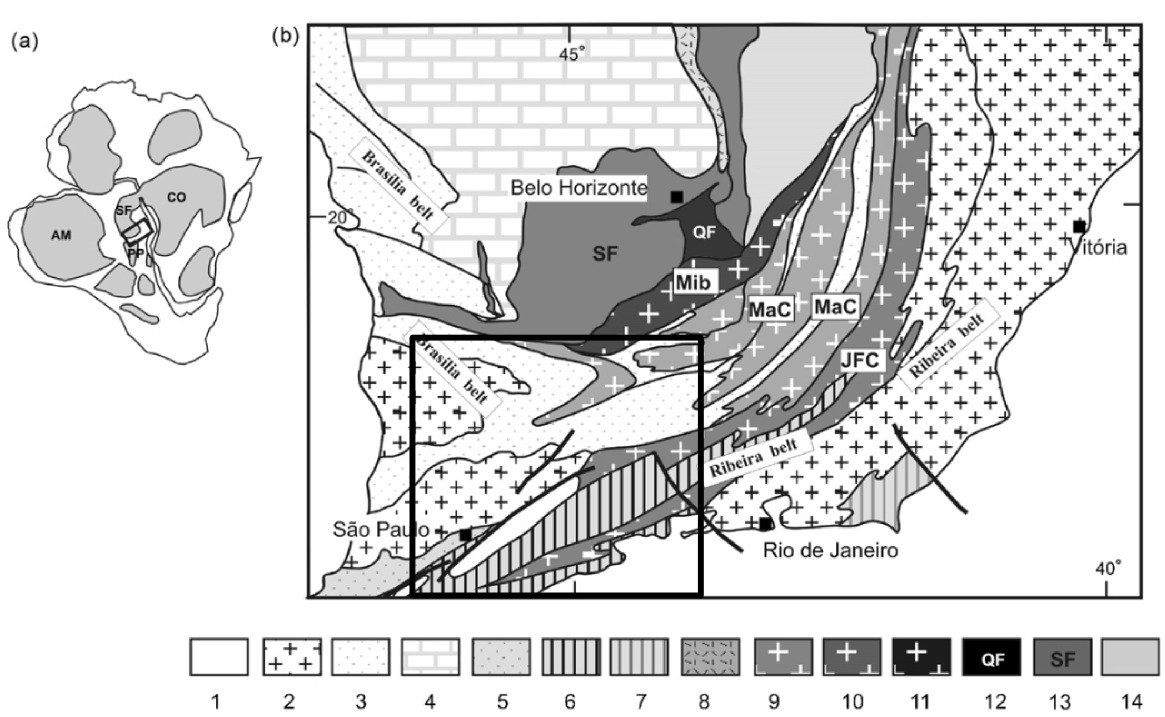
\includegraphics[scale=0.5]{Figs/mapa_geologico.png}
\caption[Mapa tectônico da Região do Sudeste do Brasil segundo  \cite{trouw_new_2013}.]{Mapa tectônico da Região do Sudeste do Brasil com a área de trabalho marcada pelo quadradro. Legenda: 1-Bacias do Paraná e do Rift Cenozóico. 2-Plutons alcalinos Cenozóicos/Cretácios. Cráton São Francisco e Bacias interiores (3–5), 3-Embasamento; 4-Cobertura (Grupo Bambuí); 5-Cobertura (rochas metasedimentares autóctones e paraautóctones. Orógeno Brasília (6-9) 6-Sistema de \textit{Nappe} Andrelândia(AND) e \textit{Nappe} Passos(P);7-\textit{Nappe} Socorro(S)-Guaxupé(G); 8- Terreno Embu(E)-Paraíba do Sul(PS); 9-Terreno Apiá. Orógeno Ribeira(6-14), 10-Domínio Externo; 11- Domínio Juiz de Fora; 12-Arco Rio Negro(Terreno Oriental); 13-Terreno Oriental; 14- Terreno Cabo Frio. A área demarcada com a linha tracejada cobrindo a parte sul da Faixa Brasília e a parte sudeste do Cráton São Francisco corresponde a uma zona de interferência onde a deformação e o metamorfismo da Faixa Ribeira se  sobressai na Faixa Brasília. Adaptado de \cite{trouw_new_2013}}
\label{mapa_geologico}
\end{figure} 

O sul da Faixa Brasilía foi descrito, \cite{pimentel_tectonic_2011},\cite{reno_situ_2012} e \cite{trouw_new_2013}, como resultado da colisão entre a margem passiva do paleocontinente São Francisco do leste com a margem ativa do bloco, ou paleocontinente, Paranapanema do lado oeste da sutura, observado no perfil A-B na Figura \ref{perfil_esquematico}. Esta colisão produziu um empilhamento espesso de \textit{nappes} ao longo da sutura, como o Sistema de \textit{Nappe} Andrelândia(ANS), que pode ser observado nos perfis mostrados no perfil A-B mostrado na Figura \ref{perfil_esquematico}. Dobras em bainha em grande escala e inúmeras dobras interropidas atestam a deformação dúctil intensa dentro das \textit{Nappes}. Lineamentos alongado, combinados com indicadores de cisalhamento mostram do norte para o sul a troca progressiva, cavalgando do topo para E-SE  na \textit{Nappe} Passos. A sutura desse cinturão é interpretada sendo localizada entre a \textit{Nappe} Socorro-Guaxupé e o Sistema \textit{Nappe} Andrelândia, como mostrado no perfil C-D na Figura \ref{perfil_esquematico}.

\begin{figure}[!ht]
\centering
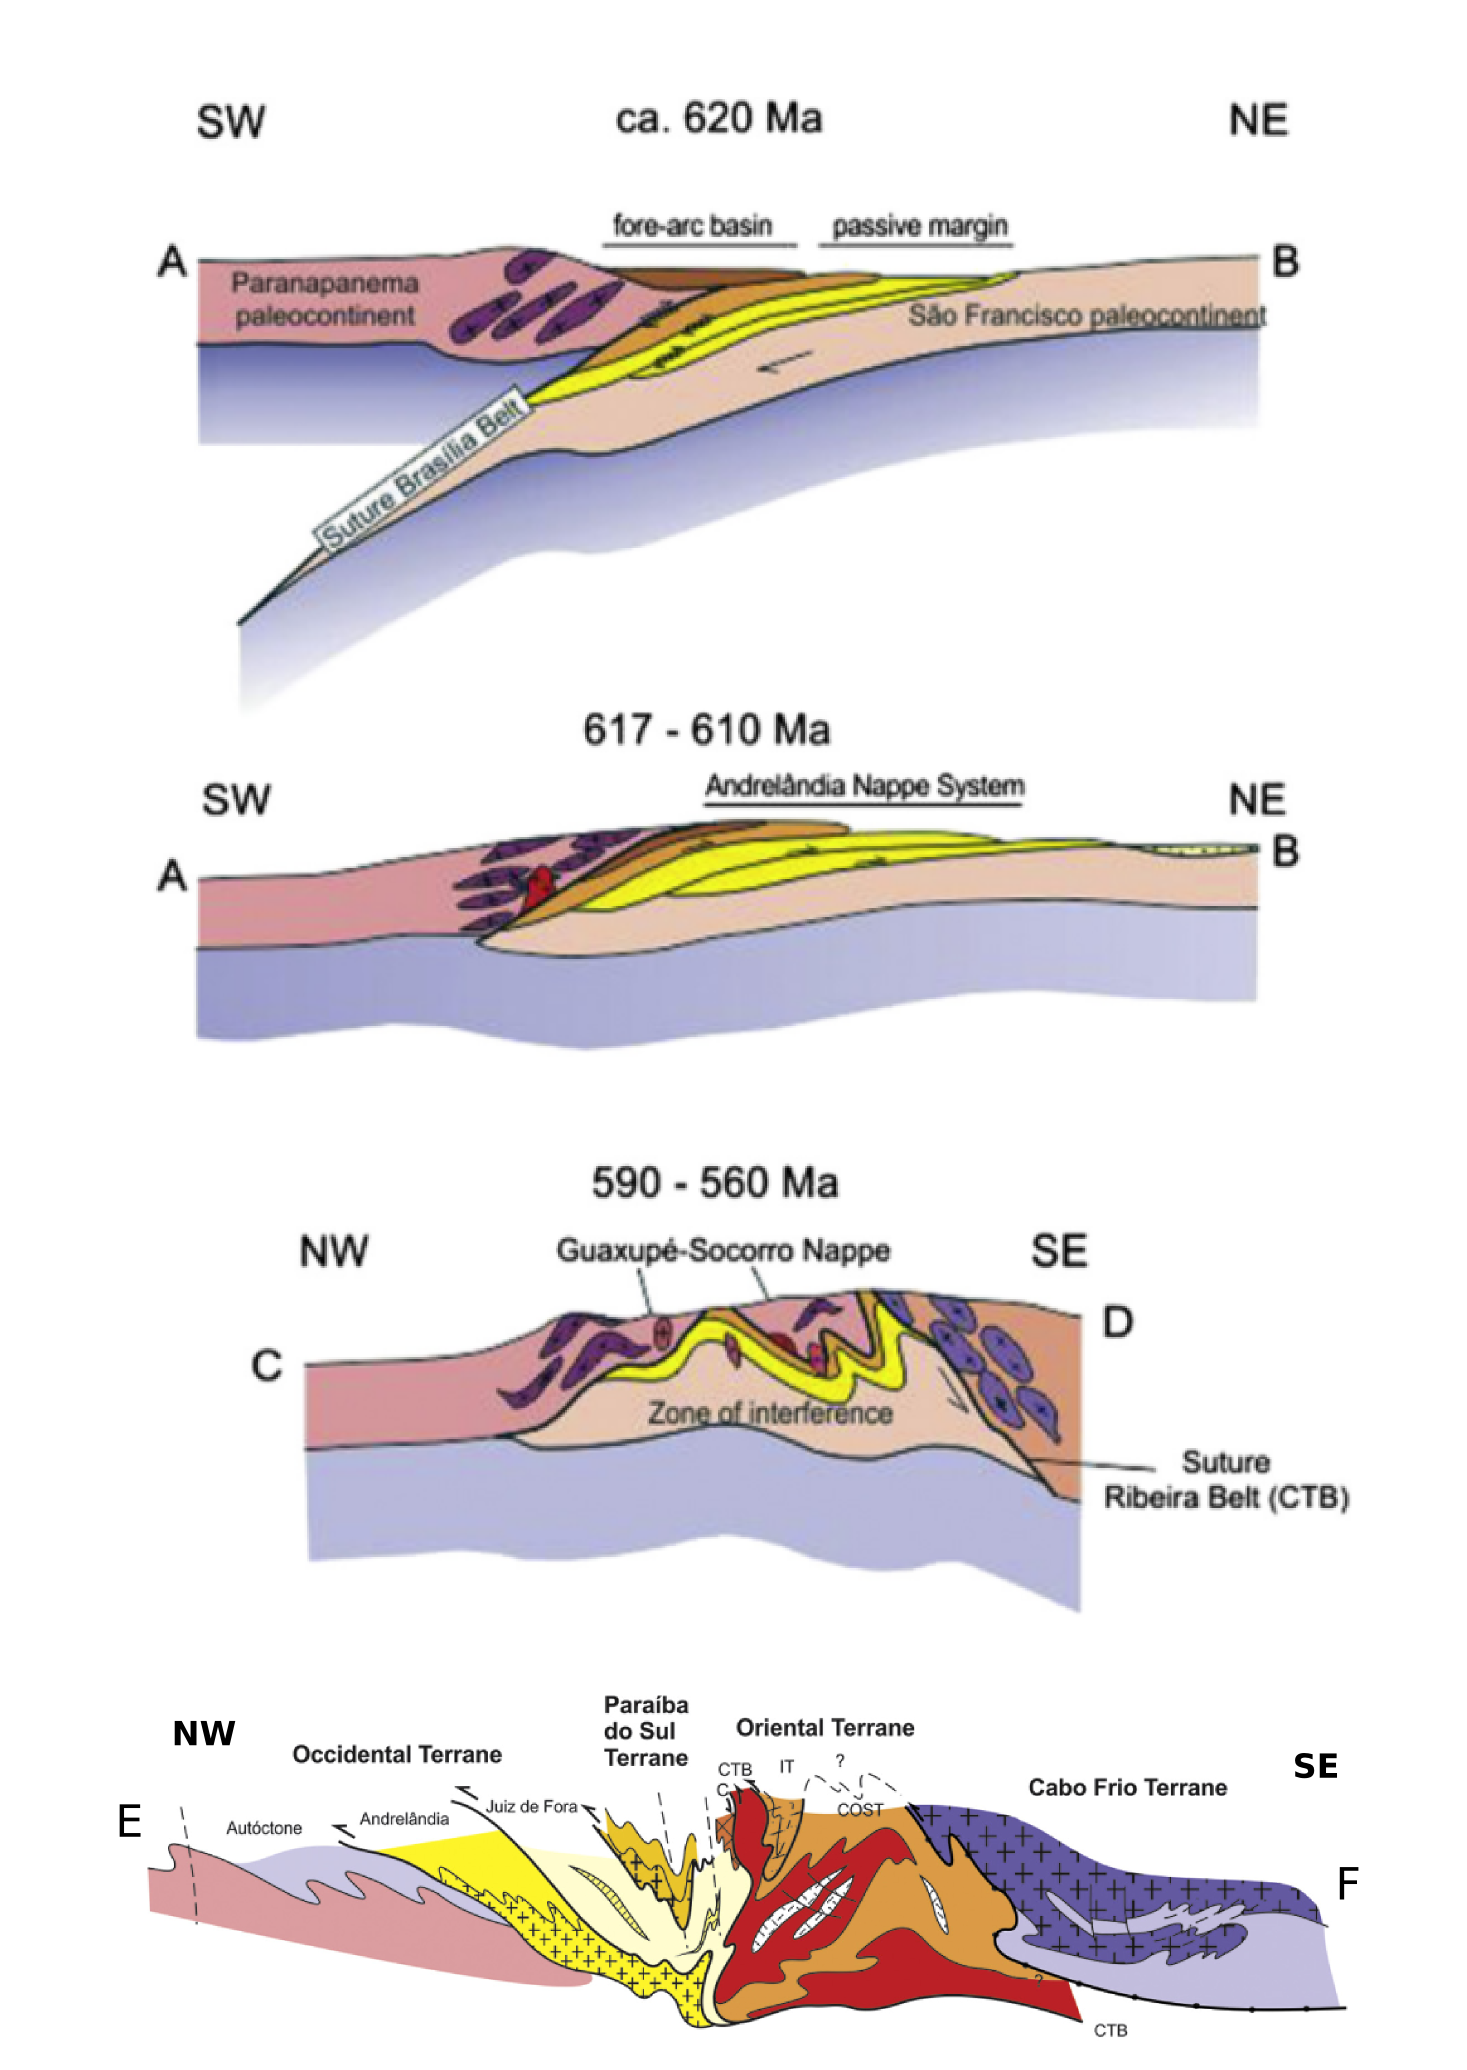
\includegraphics[scale=0.5]{Figs/perfil_esquematico_area.png}
\caption[Perfis Esquemáticos da Região do Sudeste do Brasil segundo  \cite{trouw_new_2013}.]{Perfis Esquemáticos marcados na Figura \ref{mapa_geologico} mostrando a evolução da superposição na zona de interferência. Retirado de \cite{trouw_new_2013}}
\label{perfil_esquematico}
\end{figure} 

A Faixa Ribeira é composta por rochas metamórficas, migmatitos e granitóides relacionados ao Ciclo Orogenético Brasiliano, como citam \cite{kuhn_metamorphic_2004}, \cite{heilbron_evolution_2010} e \cite{valeriano_u_pb_2011}. Esta tendência estrutural regional NE-SW pode ser observada na Figura \ref{mapa_geologico}. Segundo \cite{heilbron_evolution_2010} a Faixa Ribeira é composta por 4 terrenos tectônicos-estratigráficos separados por falhas de
empurrão ou por zonas de cisalhamento oblíquas transpressivas: (a) a margem retrabalhada do Cráton São Francisco definida como Terreno Ocidental; (b) O Terreno Paraíba do Sul-Embú que está cavalgando sobre o Terreno Ocidental;(c) O Terreno Oriental (Serra do Mar) que inclui o Arco Magmático Neoproterozóico, e (d) O Terreno Cabo Frio, que foi acrescionado depois, por volta de 520 M.a. Estes Terrenos estão demarcados na Figura \ref{mapa_geologico}. Estes são subdivididos em vários domínios, tais domínios são identificados devido ao seu contraste litológico, geoquímica isotópica e geocronologia, cita \cite{kuhn_metamorphic_2004}. A sutura entre o Terreno Ocidental e Oriental é uma zona de cisalhamento mergulhando para noroeste (NW), também chamada de Limite Tectônico Central, \textit{Central Tectonic Boundary}(CTB) por \cite{heilbron_evolution_2010} e \cite{trouw_new_2013}, demarcada na Figura \ref{mapa_geologico}. Essa sutura pode ser mapeada continuamente por pelo menos 200 km entre a costa de São Paulo e a Serra do Órgãos, no estado do Rio de Janeiro. 

\cite{trouw_new_2013} sumariza as principais características dos terrenos que compõem a Faixa Ribera. O Terreno Ocidental é caraterizado por rochas do embasamento Paleoproterozóico a Arqueano, representado pelos Complexos Barbacena, Mantiqueira e Juiz de Fora, e por uma cobertura siliciclástica metamorfizada oriunda de uma margem passiva. Esta é chamada de Megassequência Deposicional Andrelândia. Já o Terreno ou Klippe Paraíba do Sul possui ortognaisses granodioríticos a graníticos do Complexo Quirino, de idade Paleoproterozóica e é coberta por rochas do Complexo Paraíba do Sul, gnaisses feldspáticos e pelíticos, com intercalações de mármores dolomíticos. O Terreno Oriental aloja ortognaisses tonalíticos a granodioríticos pertencentes ao Complexo Rio Negro, bem como metassedimentos Neoproterozóicos, ricos em intercalações carbonáticas e rochas metabásicas. A Colisão deste terrenos acarretou na geração de vários tipos de rochas granitóides sin-colisionais: leucogranitos, charnockitos, granitos porfiróides e bitotita granitos. Por fim, o Terreno Cabo Frio engloba ortognaisses Paleoproterozóicos do Complexo Quirino e uma sucessão metassedimentar com gnaisses pelíticos com cianita, sillimanita e granada, metabasitos e rochas calcissilicáticas. 

\begin{figure}[!ht]
\centering
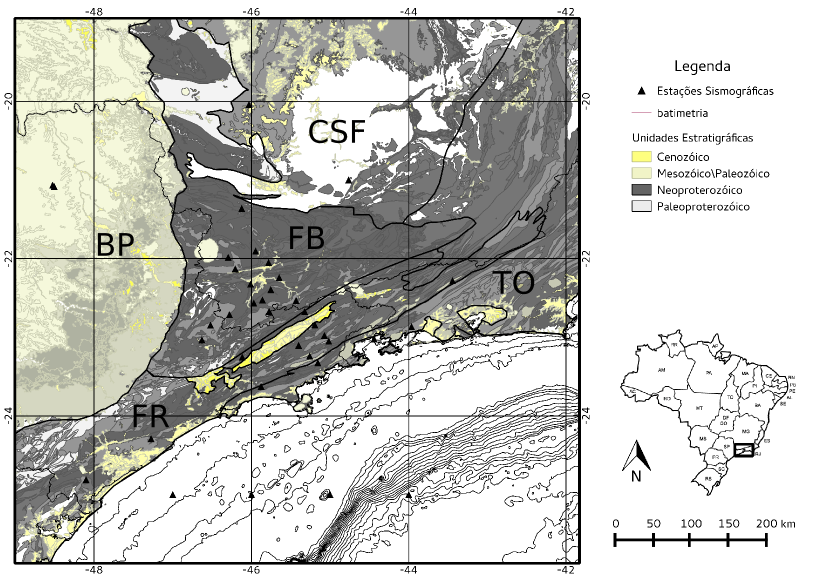
\includegraphics[scale=0.5]{Figs/mapa_estacoes_geologico.png}
\caption[Mapa de localização das Estações Sismográficas na região com o mapa geológico simplificado.]{Mapa de localização das Estações Sismográficas utilizadas neste trabalho e o mapa simplificado das unidades estratigráficas e tectônicas. BP-Bacia do Paraná, CSF-Cráton São Francisco, FB-Faixa Brasília, FR-Faixa Ribeira, TO-Terreno Oriental.}
\label{mapa_estacoes_geologico}
\end{figure}


\chapter*{Metodologia}

\section*{Função do Receptor}
\subsection*{Aquisição de Dados}

No âmbito do projeto SUBSAL, realizado conjuntamente entre o Observatório Nacional e a Petrobras,  instalou-se 24 estações sismográficas temporárias banda larga (STS2 ou Reftek RT151-120s). A faixa de frequência registrada varia de 50 Hz até 100 segundos.  As estações foram dispostas espacialmente em trẽs perfis em relação à costa, dois perpendiculares à costa, perfil 1 a oeste e perfil 2 a leste, e um paralelo, perfil 3, como observado na Figura \ref{map_loc}. O perfil 1 estende-se da estação STA01, localizada próximo à costa, até a STA09. O perfil 2 vai da estação STA10, ao norte, até a STA16, próximo à costa. O perfil 3 é da estação STA17, oeste, até a STA24, leste. A distância entre as estações é aproximativamente de 20 km. As coordenadas das estações são dadas na Tabela \ref{tabela1}. 

\begin{figure}[!ht]
\centering
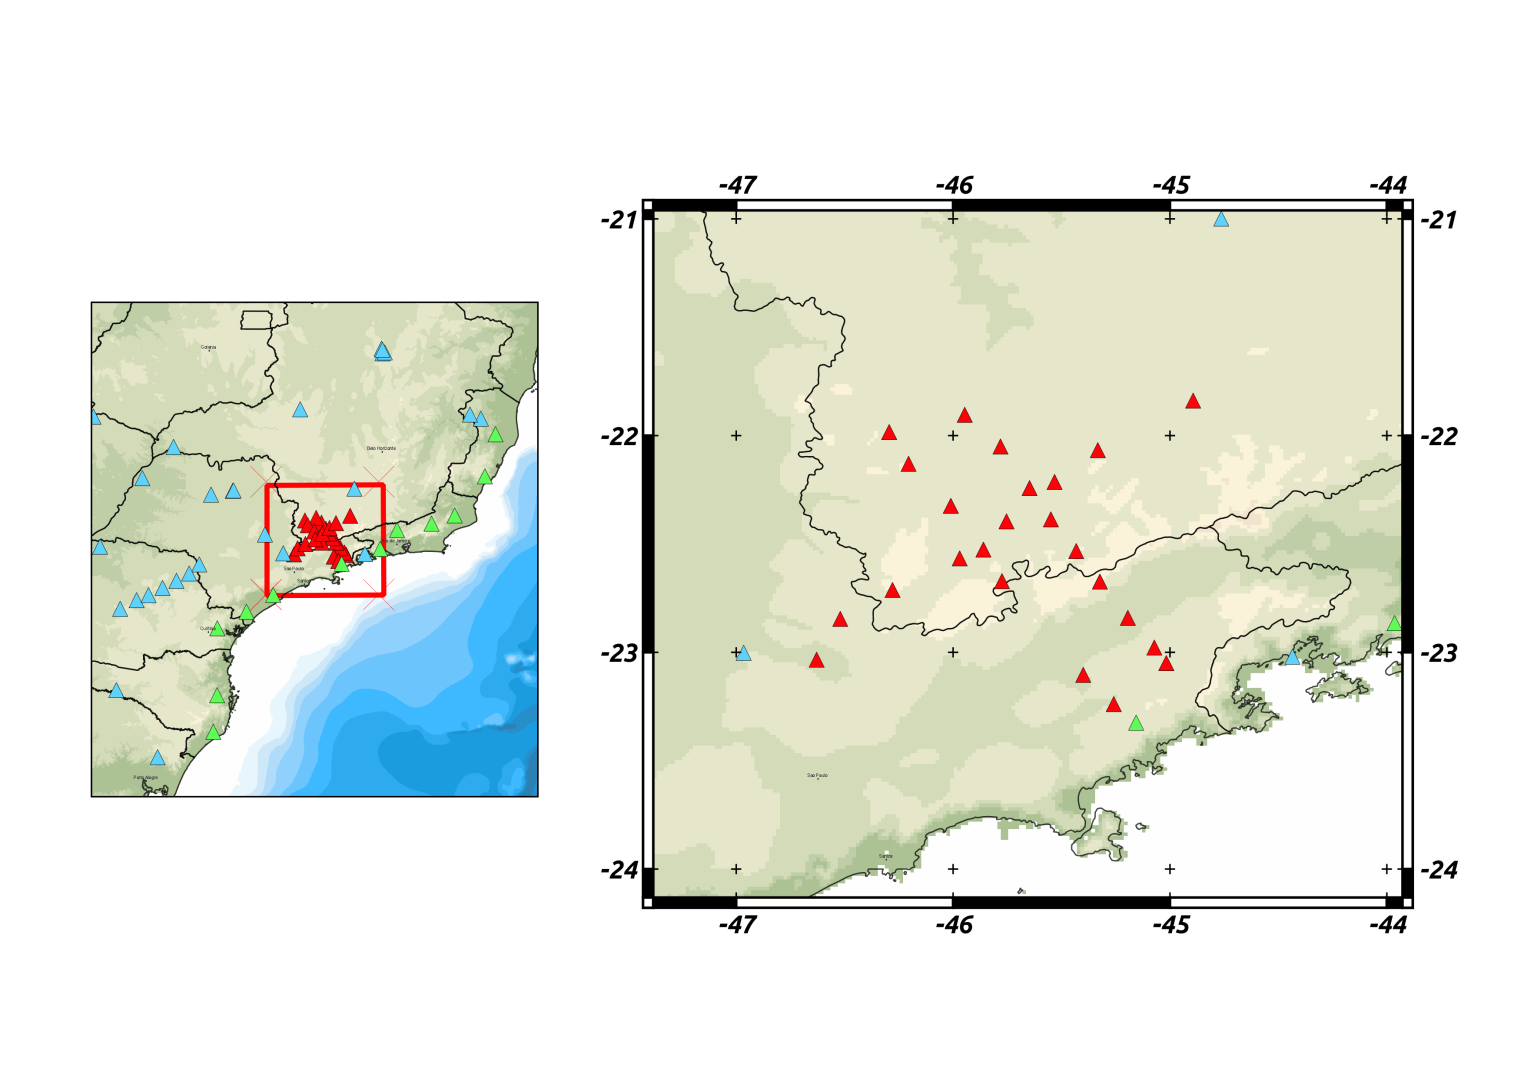
\includegraphics[scale=0.4]{mapa_das_estacoes_simosgraficas_instaladas.png}
\caption{Mapa das estações sismográficas instaladas (triângulos vermelhos). Os outros triângulos são estações da Rede Sismográfica Brasileira.}
\label{map_loc}
\end{figure}

O período de operação das estações foi distinto para os perfis. Os dois perfis perpendiculares à costa foram instalados no meio do ano de 2012 e o perfil paralelo no final de 2012. As estações ficaram em fucionamento até o final do ano de 2013 registrando o movimento do terreno de maneira contínua. 

O produto do deslocamento das partículas do meio registrado pelo sismógrafo, através de sensores verticais e horizontais em três componentes, pode ser visto na Figura \ref{simograma}. Esse registro da variação da amplitude em uma série temporal é chamado de sismograma. 

\begin{figure}[!ht]
\centering
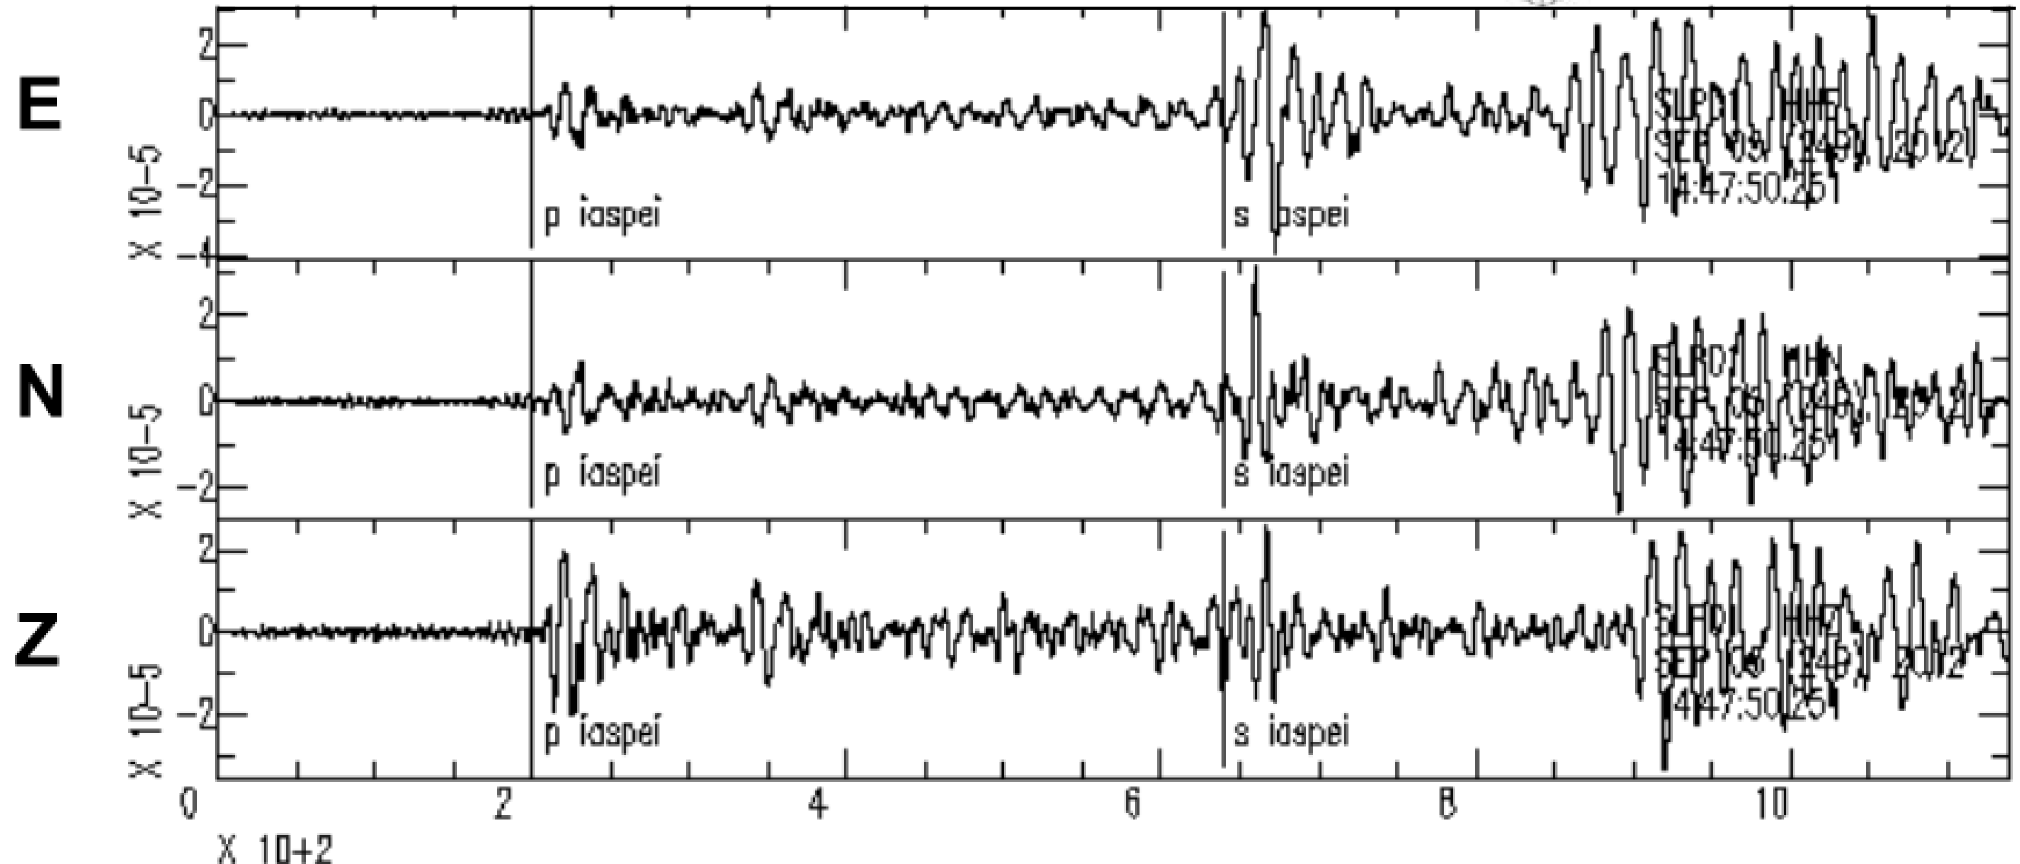
\includegraphics[scale=0.6]{sismograma.png}
\caption{Sismograma mostrandos as três componentes do deslocamento do terreno.}
\label{simograma}
\end{figure}

O sismograma é gerado pela perturbação do meio pelas ondas  mecânicas que se propagam no interior da Terra. Essas ondas  tem velocidades variando em função dos parâmetros elásticos do meio e da densidade. E estes variam pela mineralogia e condições de pressão e temperatura do meio atravessado. As ondas mecânicas são divididas em ondas de corpo e de superfície. As ondas de corpo estão categorizadas em dois tipos: as ondas P, longitudinal, e as ondas S, transversais. A onda P é mais rapida e que consegue se propagar em todos os meios, tem velocidade entre 4 e 7 km$/$s na crosta terrestre e em torno de 8 km$/$s no manto superior. As ondas S tem velocidade menor do que a onda P, em torno de 3 a 4 km$/$s na crosta.

Para produzir esta análise sobre a estrutura da região de estudo utilizou-se de um conjunto de dados com eventos sísmicos registrados. O número de eventos utilizados no processamento varia devido ao nível de sinal-ruído da forma da onda, pois há uma necessidade de visualização clara da chegada da onda P, como pode ser constatado na Figura \ref{simograma} .

\subsection*{Pré-processamento}

Para assegurar a confiabilidade do processamento é necessário um tratamento preliminar dos sinais brutos. Utilizou-se eventos catalogados na rede IRIS para uma identificação automática nestes sinais. Alguns pré-requisitos foram utilizados para a escolha dos eventos, como:

\begin{enumerate}
\item Distância Epicentral;
\item Magnitude;
\end{enumerate}

Sismos próximos, com distância menor que 20 graus da estação estudada, geram ondas com incidência oblíqua e esse tipo de dado deve ser utilizado com cuidado. Em sismos com distâncias maiores que 95 graus as ondas P não chegam na estação devido a inversão de velocidade no limite manto-núcleo, diminuição da velocidade da onda P entre o manto e o núcleo, e não é observada a onda P direta. Por isso a distância epicentral é tida como ideal entre 20 e 95 graus, como é observado na Figura \ref{mapa_eventos}. Devido grande parte dos sismos serem oriundos da Cordilheira dos Andes,como é visto na Figura \ref{teste_tempo}, também utilizou-se dados comn distância menor que 20 graus. A magnitude do sismo é importante para a propagação da onda, eventos com pequena magnitude não tem energia suficiente para gerar energia suficiente para gerar um sinal claro no sismograma.

\begin{figure}[!ht]
\centering
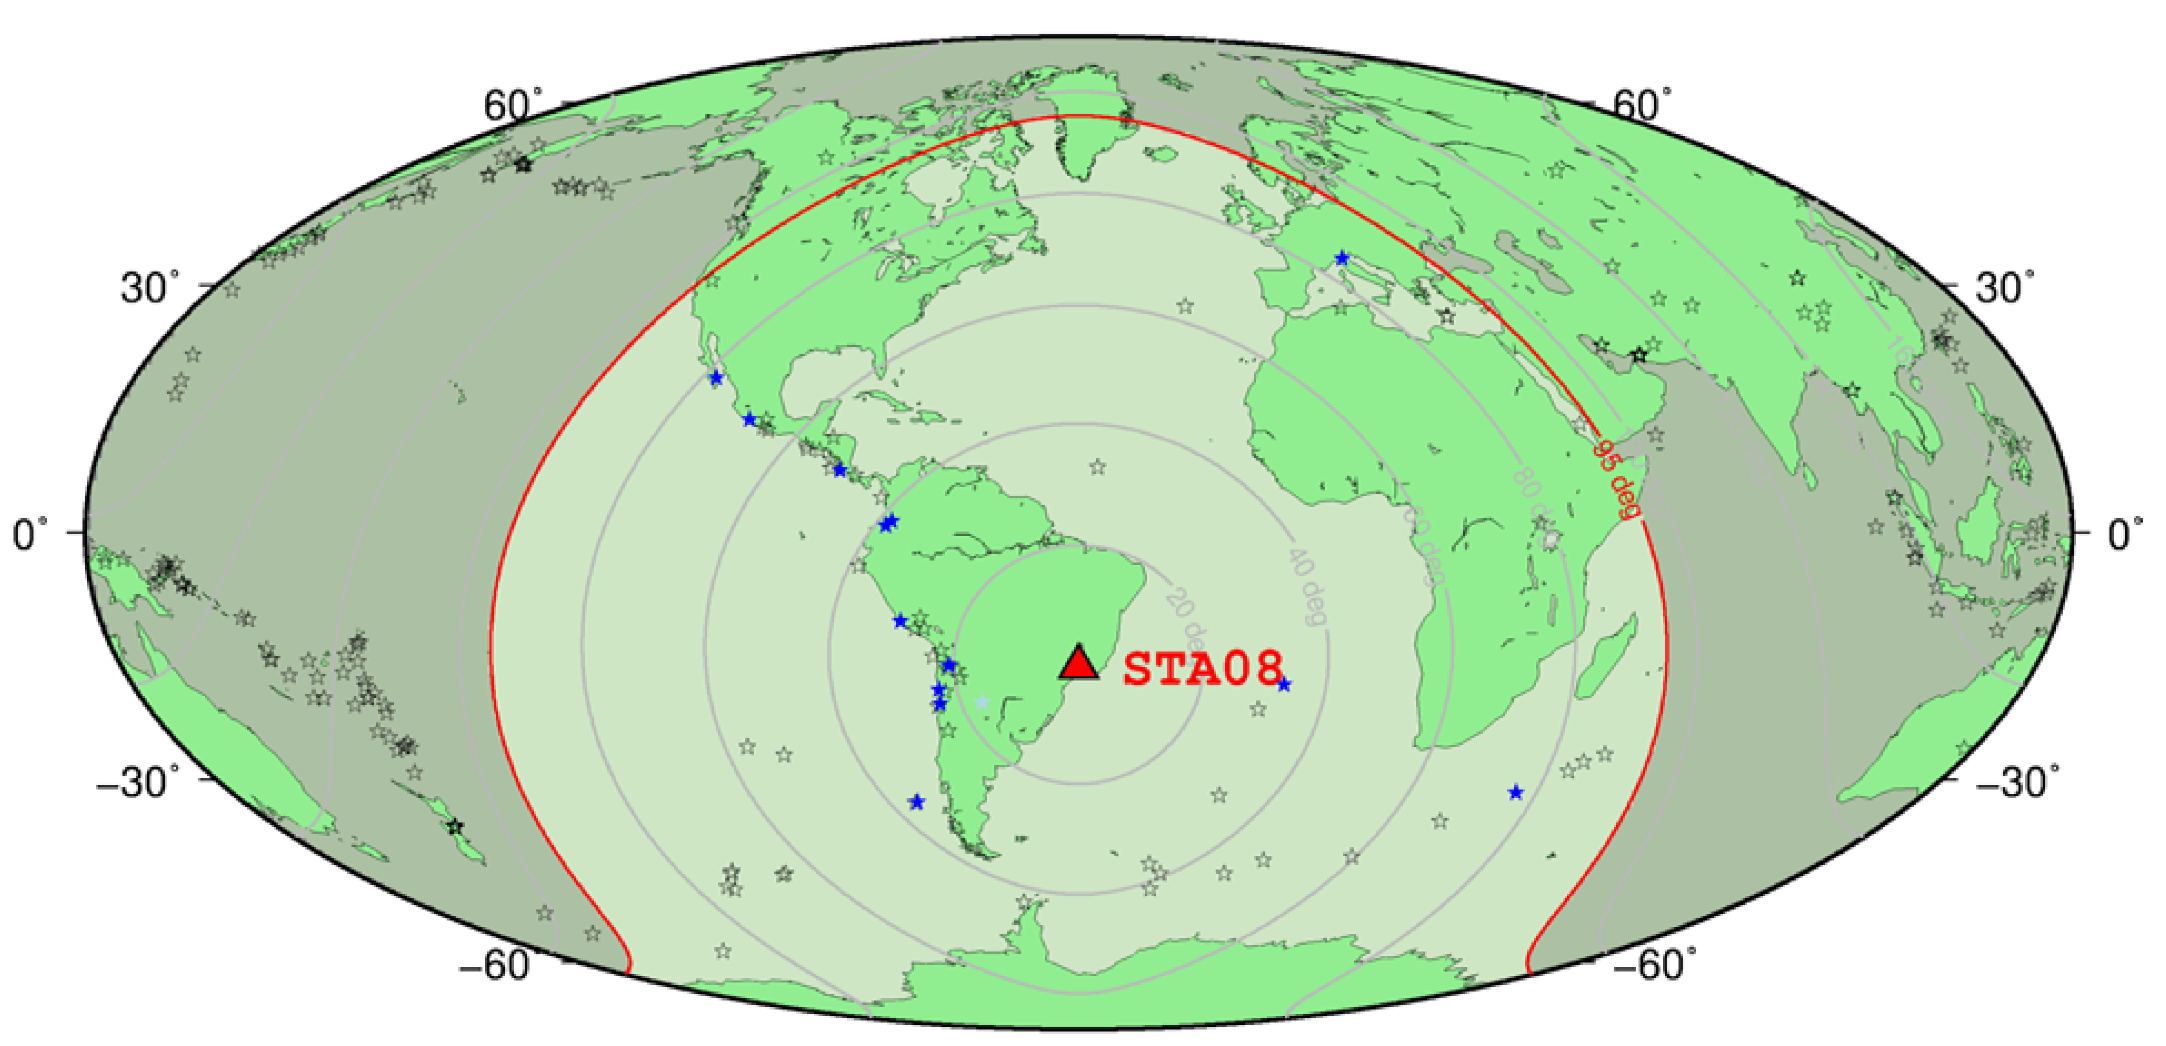
\includegraphics[scale=0.6]{mapa_de_eventos.png}
\caption{Mapa dos eventos (estrelas) registrados na estação STA08. O limite de 95 graus está indicada em vermelho. Estrelas azuls mostram os eventos com dados de qualidade que são usadas no calculo das Funçoes do Receptor}
\label{mapa_eventos}
\end{figure}


Subsequentemente um janelamento do registro em 5 segundos antes e 10 segundos depois da chegada da onda P, esta é calculada pelo modelo de velocidade da Terra  IASPEI91 \citep{kennet_iaspei_1991}. Após a discriminação e o janelamento do sinal, examina-se visualmente cada registro para certificar que todos os eventos selecionados tem um nível de sinal-ruído bom, como na Figura \ref{simograma} . 

Logo após removeu-se a média e tendência linear dos dados. Aplicou-se um filtro passa-alta com freqüência de corte de 0.1 Hz para eventos com distância entre 20 e 95 graus e de 2 Hz para eventos próximos (<20). Os dados originais com amostragens a cada 0,01 segundos (100 Hz) são interpolados para gerar dados com amostragens cada 0,025 segundas (40 Hz), porque a informação de alta freqüência não é relevante nesse tipo de análise.

\subsection*{Processamento}

A caracterização prévia das informações contidas no sinal é imprescindível para o processamento. A avaliação da performance e da qualidade dos dados da estações sismográficas foram feitas no software livre PQLX.  A metodologia do PQLX é baseada no trabalho de \cite{McNamara_Buland_2004}. Esse procedimento é bastante usado para se obter a informação espectral sísmica.

No programa PQLX a série temporal é segmentada em intervalos de uma hora, com 50\% de superposição do sinal. Cada janela de hora está separada em 13 intervalos com 75\% de superposição para calcular a “Power Spectral Density”. As médias obtidas para cada um dos 13 intervalos são usadas para estimar a “Probability Density Functions”, calculados a partir das médias pelo número total de segmentos de hora em hora. 

Essa metodologia de \cite{McNamara_Buland_2004} difere dos métodos habitualmente utilizados, porque não é necessário a visualização de todo conjunto de dados para uma estima qualitativa do sinal, observado na Figura \ref{PQLX}.

\begin{figure}[!ht]
\centering
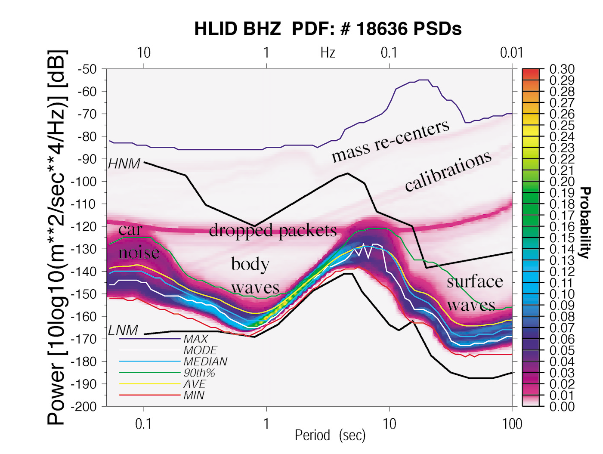
\includegraphics[scale=0.8]{mcnamura_buland.png}
\caption{Análise qualitativa do sinal atraves das \textit{Power Density Functions}. \cite{McNamara_Buland_2004} }
\label{PQLX}
\end{figure}

A garantia da fiabilidade do tempo de chegada da onda P é fundamental para o processamento gerar resultados consistentes. Portanto testes com o tempo de chegada da onda P forão feitos. \cite{gibbons_identification_2006} mostra que fazendo a correlação de dois eventos distantes em uma estação sismográfica consegue-se caracterizar esse tempo de chegada, como é visto na Figura \ref{teste_tempo}. \cite{gibbons_identification_2006} assume que  se não há alterações mensuráveis na velocidade da estrutura entre a fonte e os receptores, ondas sísmicas de dois eventos co-localizados terá a mesma duração de tempo para chegar a um determinado sensor. A função de correlação cruzada para um dado sinal a uma dada estação mede que a semelhança entre a porção posterior do sismograma é a do modelo de forma de onda. O tempo de separação entre o início do modelo e o valor máximo da função de correlação cruzada deve ser igual ao tempo que separa os dois tempos de origem dos eventos para todas as estações. Qualquer discrepância nos tempos de separação medido em duas estações diferentes, o que não é atribuível a diferença entre fontes ou uma SNR baixa, deve ser o resultado de uma anomalia em sincronismo um, ou ambos, dos instrumentos.

Nesste trabalho utilizamos uma metodologia semelhante a de \cite{gibbons_identification_2006}. Utilizou-se um sismo distante de um par de estações sismográficas próximas. Com os sinais registrados fez-se a correlação cruzada dos dados. Como a fonte está distante das estações a correlação dos sinais deve ser próxima de zero. Este teste do tempo de chegada da onda P é para garantir a confiabilidade dos dados das estações temporárias. Portanto em cada par de estações correlacionadas sempre tinha uma estação permanente, estação com dados confiáveis.

\begin{figure}[!ht]
\centering
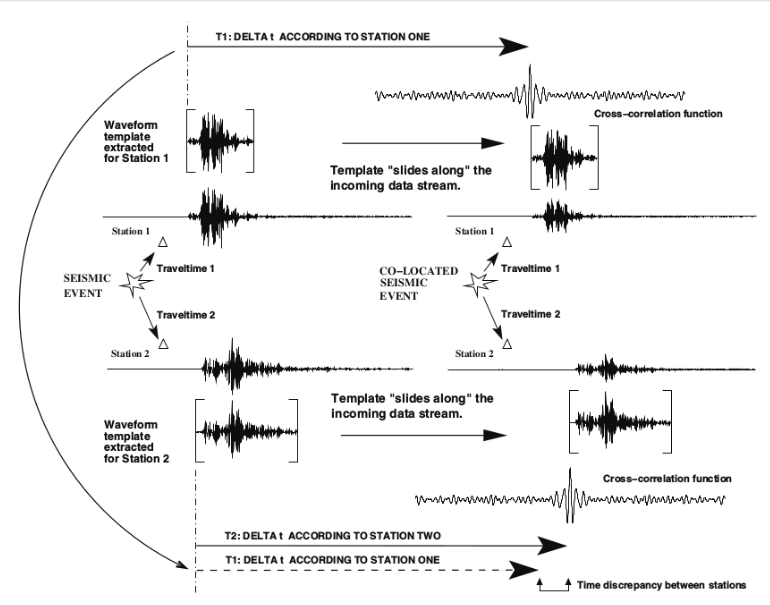
\includegraphics[scale=0.6]{correlacao_tempo_de_chegada.png}
\caption{Uma ilustração esquemática de como dois eventos sucessivos de fontes sísmicas quase idênticas que podem ser explorados para revelar anomalias dos tempo de chegada da onda P numa dada estação. \citep{gibbons_identification_2006}}
\label{teste_tempo}
\end{figure}

No ínicio desse trabalho somente os dados de eventos incluídos no catálogo do IRIS (\textit{Incorporated Research Institutions for Seismology}) com magnitude maior que 5,5 entre maio de 2011 e maio de 2012 foram utilizados. Porém agora utiliza-se dados coletados na rede Sismográfica, mostrada na \ref{map_loc}, até o fim do segundo semestre de 2013. A Figura \ref{mapa_eventos} mostra eventos sísmicos registrados na estação STA08 mostrando a delimitação dos eventos pela distância epicentral, além de mostrar sismos com magnitude maior que 5.5 mb.

O sismômetro registra pequenas variações horizontais e verticais de amplitude das partículas do terreno na escala microscópica ao longo das direções Vertical (Z), Norte-Sul (N) e Leste-Oeste (E), chamado sistema ZNE, como observado na Figura \ref{simograma}. No entanto, o sinal bruto nas direções ZNE não está alinhado aos eixos de propagação das ondas geradas pelo sismo, logo a resposta em cada componente mostra uma sobreposição de vários tipos de ondas. Com a finalidade de isolar a contribuição de cada onda registrada nos dados, o sistema de coordenadas dos registros são rotacionadas, através do SAC (\textit{Seismic Analysis Code}), para se alinharem com os eixos de propagação das ondas através da seguinte matriz de rotação:

\begin{eqnarray} \label{rotação}
\left[ \begin{array}{c} R \\ T \\ Z \end{array} \right] = \begin{bmatrix} \cos \theta & \sin \theta & 0 \\ - \sin \theta & \cos \theta & 0 \\ 0 & 0 & 1 \end{bmatrix} \left[ \begin{array}{c} E \\ N \\ Z \end{array} \right]
\end{eqnarray}


O resultado da equação \ref{rotação} discrimina claramente a contribuição de cada componente  no sismograma. A componente N (norte-sul) transforma-se na componente T (transversal) e guarda os registro da componente horizontal da onda S, chamada de onda SH. A resposta da onda SV é resgistrada na componente radial do sismograma, chamada R, como pode ser visualizada na Figura \ref{sismo_radial}.   

\begin{figure}[!ht]
\centering
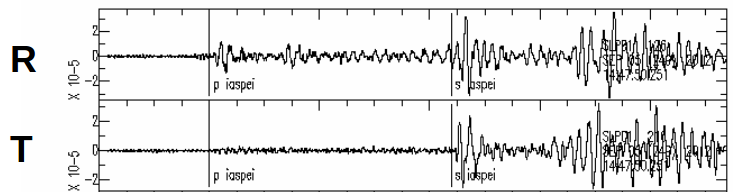
\includegraphics[scale=0.6]{Componente_Radial_Transversal.png}
\caption{Sismograma mostrando as componentes Radial e Transversal.}
\label{sismo_radial}
\end{figure}

Para o cálculo a espessura crustal na região utilizou-se o método da Função do Receptor, que foi desenvolvido por \cite{Langston_1977}. O programa SAC (\textit{Seismic Analysis Code}) foi usado para fazer o processamento e o cálculo das Funções Receptores. Tal método faz uso do sinal de tele-sismos, geradores de ondas planas de incidência quase-vertical embaixo de uma dada estação. A onda P incide na discontinuidade de Mohorovicic e se decompõe em uma onda P transmitida e uma onda S convertida. A diferença do tempo de chegada das duas ondas, onda S tem velocidade inferior a onda P, e de outras reflexões permite inferir a profundidade da discontinuidade de Mohorovicic, também chamada de Moho, como mostrado na Figura \ref{funcoes_sinteticas} .

\begin{figure}[!ht]
\centering
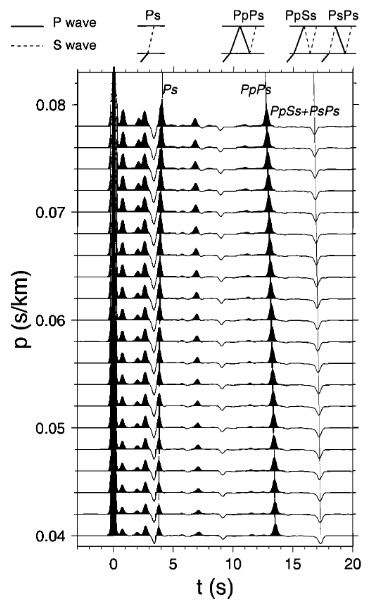
\includegraphics[scale=0.8]{funcoes_sinteticas.png}
\caption{Funções do Receptor em função do parâmetro do raio para o Modelo de Velocidade Padrão do Sul da Califórnia, em \cite{Zhu_Kanamori_2000}. A fase Ps convertida em Moho e suas múltiplas  PpPs, PpSs, e PsPs e seus traços são ilustrados no topo da imagem. Outras reflexões não-rotuladas são as conversões P-S em 5.5 km e 16 km, discontinuidades intracrustais no modelo.}
\label{funcoes_sinteticas}
\end{figure}

Para uma estimativa precisa das Funções do Receptor é essencial que o tempo de chegada da onda P seja determinado com baixa incerteza. Então os dados foram examinados visualmente para registrar o tempo de chegada da onda P direta. 

As Funções do Receptor são calculadas com uma deconvolução componente radial (R) pela componente vertical (Z), como é mostrado por \cite{clayton_source_1976}, \cite{Langston_1977}, \cite{ammon_isolation_1991}, \cite{cassidy_numerical_1992}, \cite{Zhu_Kanamori_2000}. Essa operação remove efetivamente a resposta instrumental, a assinatura da fonte e a propagação da fonte até Moho. E o sinal resultante é a assinatura da propagação próxima à estação. Então a Função do Receptor é sensível na delimitação da estruturação superficial da crosta embaixo da estação.

Computar as Funções do Receptor é um problema de deconvolução,  \cite{ligorria_iterative_1999}. \cite{langston_structure_1979} descreve a resposta do deslocamento teórico para uma onda plana P incidindo sobre uma empilhamento de interfaces horizontais ou inclinadas no domínio do tempo pode ser dada por:

\begin{eqnarray} \label{lang_equacao}
D_{V}(t) = I(t) * S(t) * E_{V}(t)
\nonumber
\\
D_{R}(t) = I(t) * S(t) * E_{R}(t)
\\
\nonumber
D_{T}(t) = I(t) * S(t) * E_{T}(t)
\end{eqnarray}

Onde $S(t)$ é a resposta efetiva da fonte em função do tempo de uma onda incidente, $I(t)$ é a resposta do impulso instrumental e $E_{V}(t)$, $E_{R}(t)$ e $E_{T}(t)$ são as respostas do impulso da estruturua vertical, radial e tangencial, respectivamente. A componente $S(t)$ pode ser muito complicada de ser computada, pois ela é relacionada a história do deslocamento no tempo e reverberações na aŕea da fonte.

\cite{langston_structure_1979} assume que eventos profundos observados em dados telessísmicos, na componente vertical do movimento do terreno ($D_{V}(t)$), se comportam como um pulso em função do tempo convoluído com a resposta instrumental e com chegadas tardias menores. Cálculos teóricos para estruturas crustais mostram que reverberações crustais e fases convertidas na componente vertical de ondas P são menores. Então se aproxima:

\begin{eqnarray} \label{lang_suposicao}
I(t) * S(t) \simeq D_{V}(t)
\end{eqnarray}

\cite{langston_structure_1979} faz uma suposição implícita que $D_{V}(t)$ comporta-se como uma função delta de Dirac, como pode ser observado na equação \ref{lang_suposicao}. Assumindo que a resposta instrumental é compensada entre as componentes, $E_{R}(t)$ e $E_{T}(t)$ podem ser encontrados passando para o domínio da frequência a equação \ref{lang_equacao} e fazendo as seguintes deconvoluções:

\begin{eqnarray} \label{lang_resposta}
E_{R}(\omega) =  \frac{D_{R}(\omega)}{I(\omega)S(\omega)} \simeq \frac{D_{R}(\omega)}{D_{V}(\omega)}
\\ \nonumber
E_{T}(\omega) =  \frac{D_{T}(\omega)}{I(\omega)S(\omega)} \simeq \frac{D_{T}(\omega)}{D_{V}(\omega)}
\end{eqnarray}

$E_{R}(t)$ e $E_{T}(t)$ são retransformadas para o domínio do tempo, importante lembrar que nessa técnica a informação da fase é conservada. \cite{langston_structure_1979} resalta que o resultado da série temporal pode ser interpretado diretamente com um sismograma, permitindo que tempo e amplitude de chegadas possam ser examinadas de uma maneira inequívoca.

Um método robusto de análise das Funções do Receptor é o método de \cite{Zhu_Kanamori_2000}. Usando as velocidades medianas na crosta, as diferenças de tempo entre a P direta e a P convertida em S podem ser calculadas, bem como os tempos das múltiplas. Usando uma dada velocidade v p , os tempos de chegada podem ser calculados usando a profundidade de Moho (H), a razão v p /v s e o parâmetro do raio, este é dependente da localização do evento e da profundidade. Ao invés de tentar ajustar toda a função, o método faz uma pesquisa, grid search, da espessura crustal e da razão v p /v s para calcular o tempo de chegada teórico das ondas P convertidas em S e das múltiplas para cada registro. A melhor combinação da espessura crustal e da razão v p /v s é aquela que maximiza o valor das amplitudes reais das funções receptor. Para obter uma imagem das discontinuidades, como por exemplo Moho, as Funções do Receptor empilhadas são mapeadas em relação a posição da estação no perfil. 

Os dados são separados em 4 grupos, segundo o azimute entre o sismo e a estação. A maioria do eventos ocorrem na região noroeste e sudoeste, nota-se a escassez de eventos na região do Oceano Atlântico. O objetivo dessa separação é avaliar se existem variações laterais de estrutura.


\section*{Dispersão de Ondas de Superfície}
\subsection*{Dados Geofísicos}
\subsection*{Fundamentos Teóricos}
\chapter{Resultados e Discussões}

Pesquisas envolvendo a propagação de ondas sísmicas no interior da Terra auxiliam na determinação da estrutura da mesma. Essas análises permitem recuperar, de acordo com a resolução, a geometria das descontinuidades de propriedades físicas terrestres, principalmente a velocidade de propagação das ondas de corpo.  

O método da Função do Receptor, desenvolvido por \cite{Langston_1977}, gera informações sobre a estrutura abaixo da estação sismográfica. A confiança nos resultados gerados pelo método varia em função da quantidade e qualidade das Funções do Receptor. Por isso é importante que a estação esteja funcionando corretamente e tenha uma grande quantidade de dados disponíveis.

Será dado enfoque as fases de função do receptor relacionadas à discontinuidade de Moho, interface Crosta-Manto, e reflexões  internas, antes de 5 segundos. Os resultados obtidos pelas estações temporárias serão comparados com a estação SLP01, estação permanente próxima a região de estudo, como mostrado na Figura \ref{RF_SLP01_STA08}. Assim aumentando a confiabilidade nos dados gerados pela rede de estações temporárias.

A Figura \ref{RF_SLP01_STA08} mostra as Funções do Receptor obtidas a partir de vários eventos na para a estação permanente SLP01 e para a estação temporária STA08, estas funções organizadas de acordo com o backazimute. Estes sinais estão normalizados pela amplitude do primeiro pico. O primeiro pick é a chegada da onda P direta, já o segundos, por volta de 5 segundos, e a onda P convertida em onda S na discontinuidade de Moho. As linhas verticais pontilhadas demarcam os tempos teóricos de chegada para cada múltipla. As multiplas $PpPs$ e $PpSs+PsPs$ tem uma amplitude menor que a onda P convertida em S($Ps$) devido a grande distância entre o ponto incidente e a estação. Então entas reverberações são mais afetadas por variações laterias, espallhamento e atenuação inelástica. Os sismosgramas não apresentam clareza quanto a essas reverberações. A múltipla $PpPs$ não é observada facilmente e a múltipla $PpSs+PsPs$ está mascarada pelo ruído.

\begin{figure}[!ht]
\centering
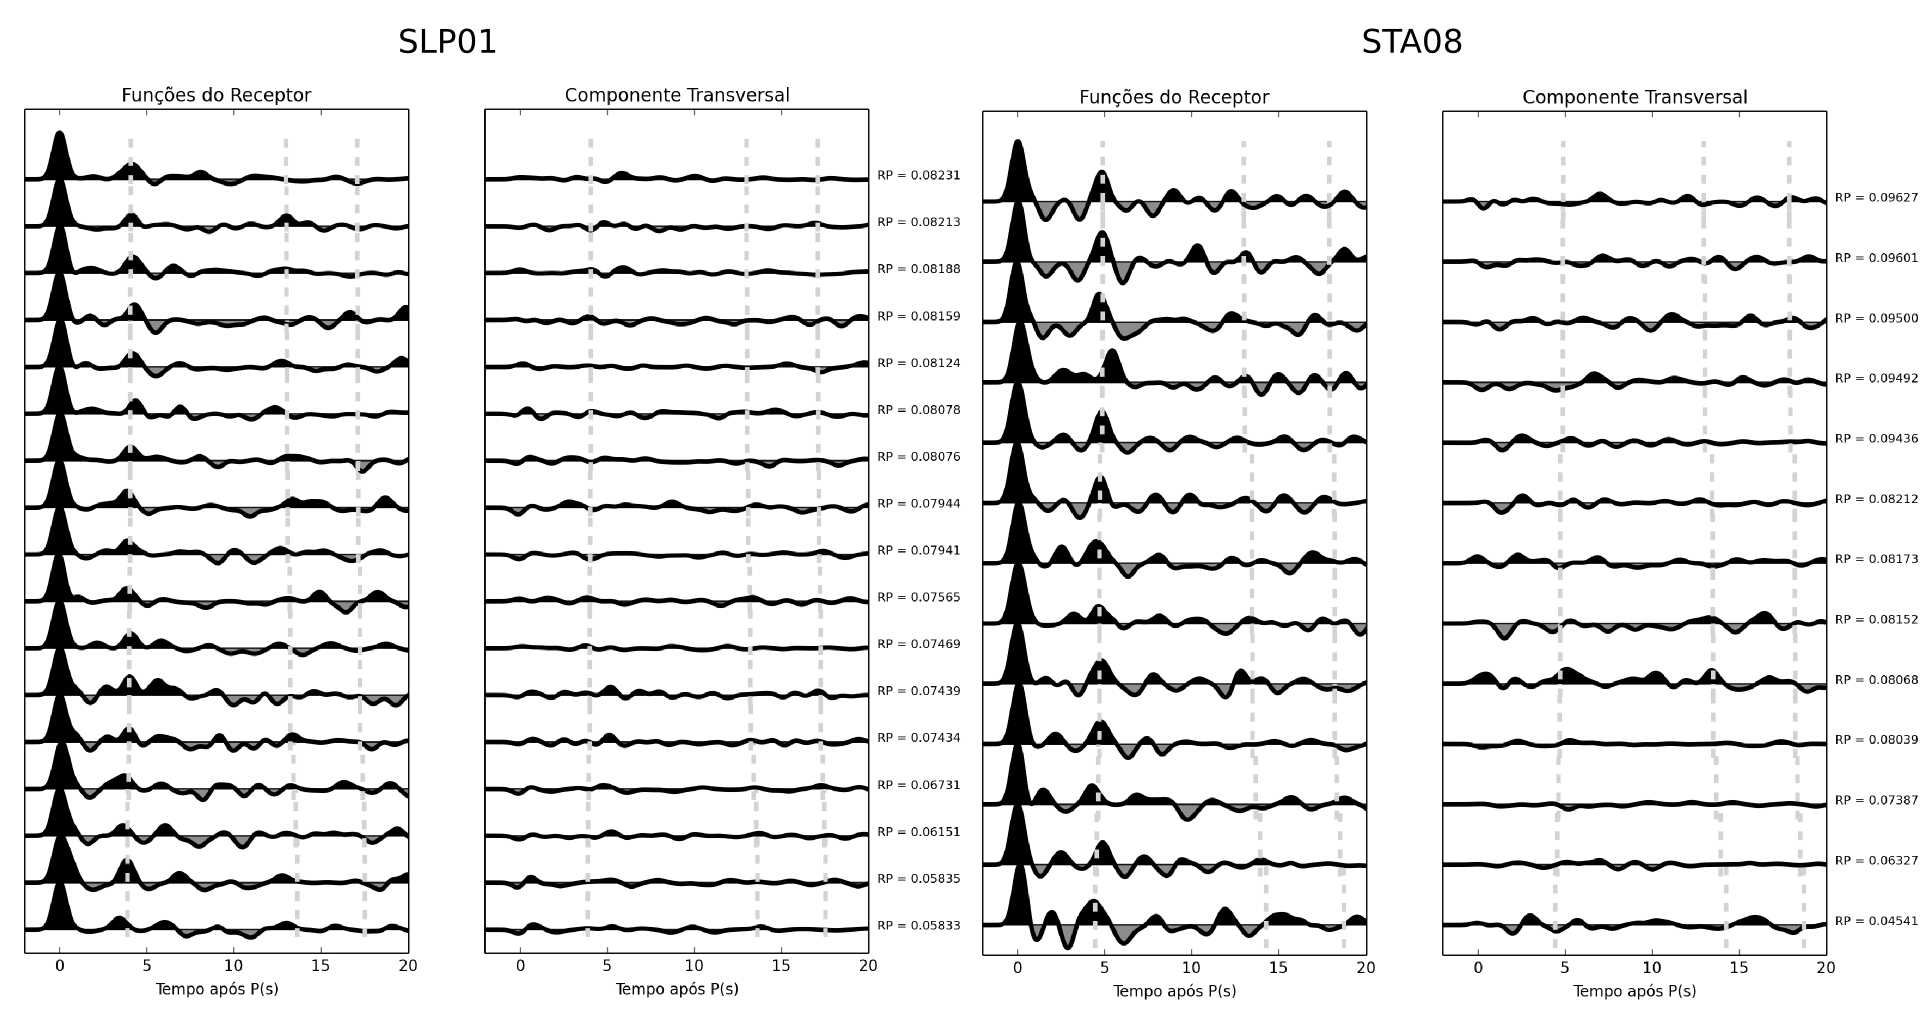
\includegraphics[scale=0.16]{Figs/RF_SLP01_STA08.png}
\caption[Exemplos de Funções do Receptor e da Componente Transversal para as estações SLP01(permanete) e STA08(temporária) distribuídas em função do parâmetro do Raio.]{Exemplos de Funções do Receptor e da Componente Transversal para as estações SLP01(permanete) e STA08(temporária) distribuídas em função do parâmetro do Raio. O primeiro pico significa a chegada da onda $P$ direta. Já o segundo a conversão da onda $P$ em $S$ em Moho. As outras múltiplas geradas em Moho não são observáveis. A linha pontilhada simboliza os tempos de chegada teóricos calculados segundo o modelo de \cite{kennet_iaspei_1991}.}
\label{RF_SLP01_STA08}
\end{figure}

DISCUSSÕES SOBRE A COMPONENTE TANGENCIAL - SAVAGE(1998)

Com as Funções do Receptor calculadas, utilizou-se a método desenvolvido por \cite{Zhu_Kanamori_2000} para calcular a profundidade de Moho e a razão $v_{p}/v_{s}$ nas estações sismográficas. Os resultados gerados estão descritos na tabela \ref{tabela1}. Para uma melhor visualização dos resultados gerados, as profundidades de Moho foram interpoladas. Para melhorar a distribuição espacial das profundidades de Moho adicionou-se dados de \cite{Assumpcao_Brazil_2013}. O mapa da interpolação pode ser visto na Figura \ref{Interpolacao}. Nota-se na Figura \ref{Interpolacao} que a discontinuidade de Moho estimada é maior no interior do continente do que na região costeira, corroborando com os dados de \cite{Assumpcao_America_2013}, \citep{Assumpcao_Brazil_2013} e \cite{van_der_meijde_gravity_2013} . 

\begin{figure}[!ht]
\centering
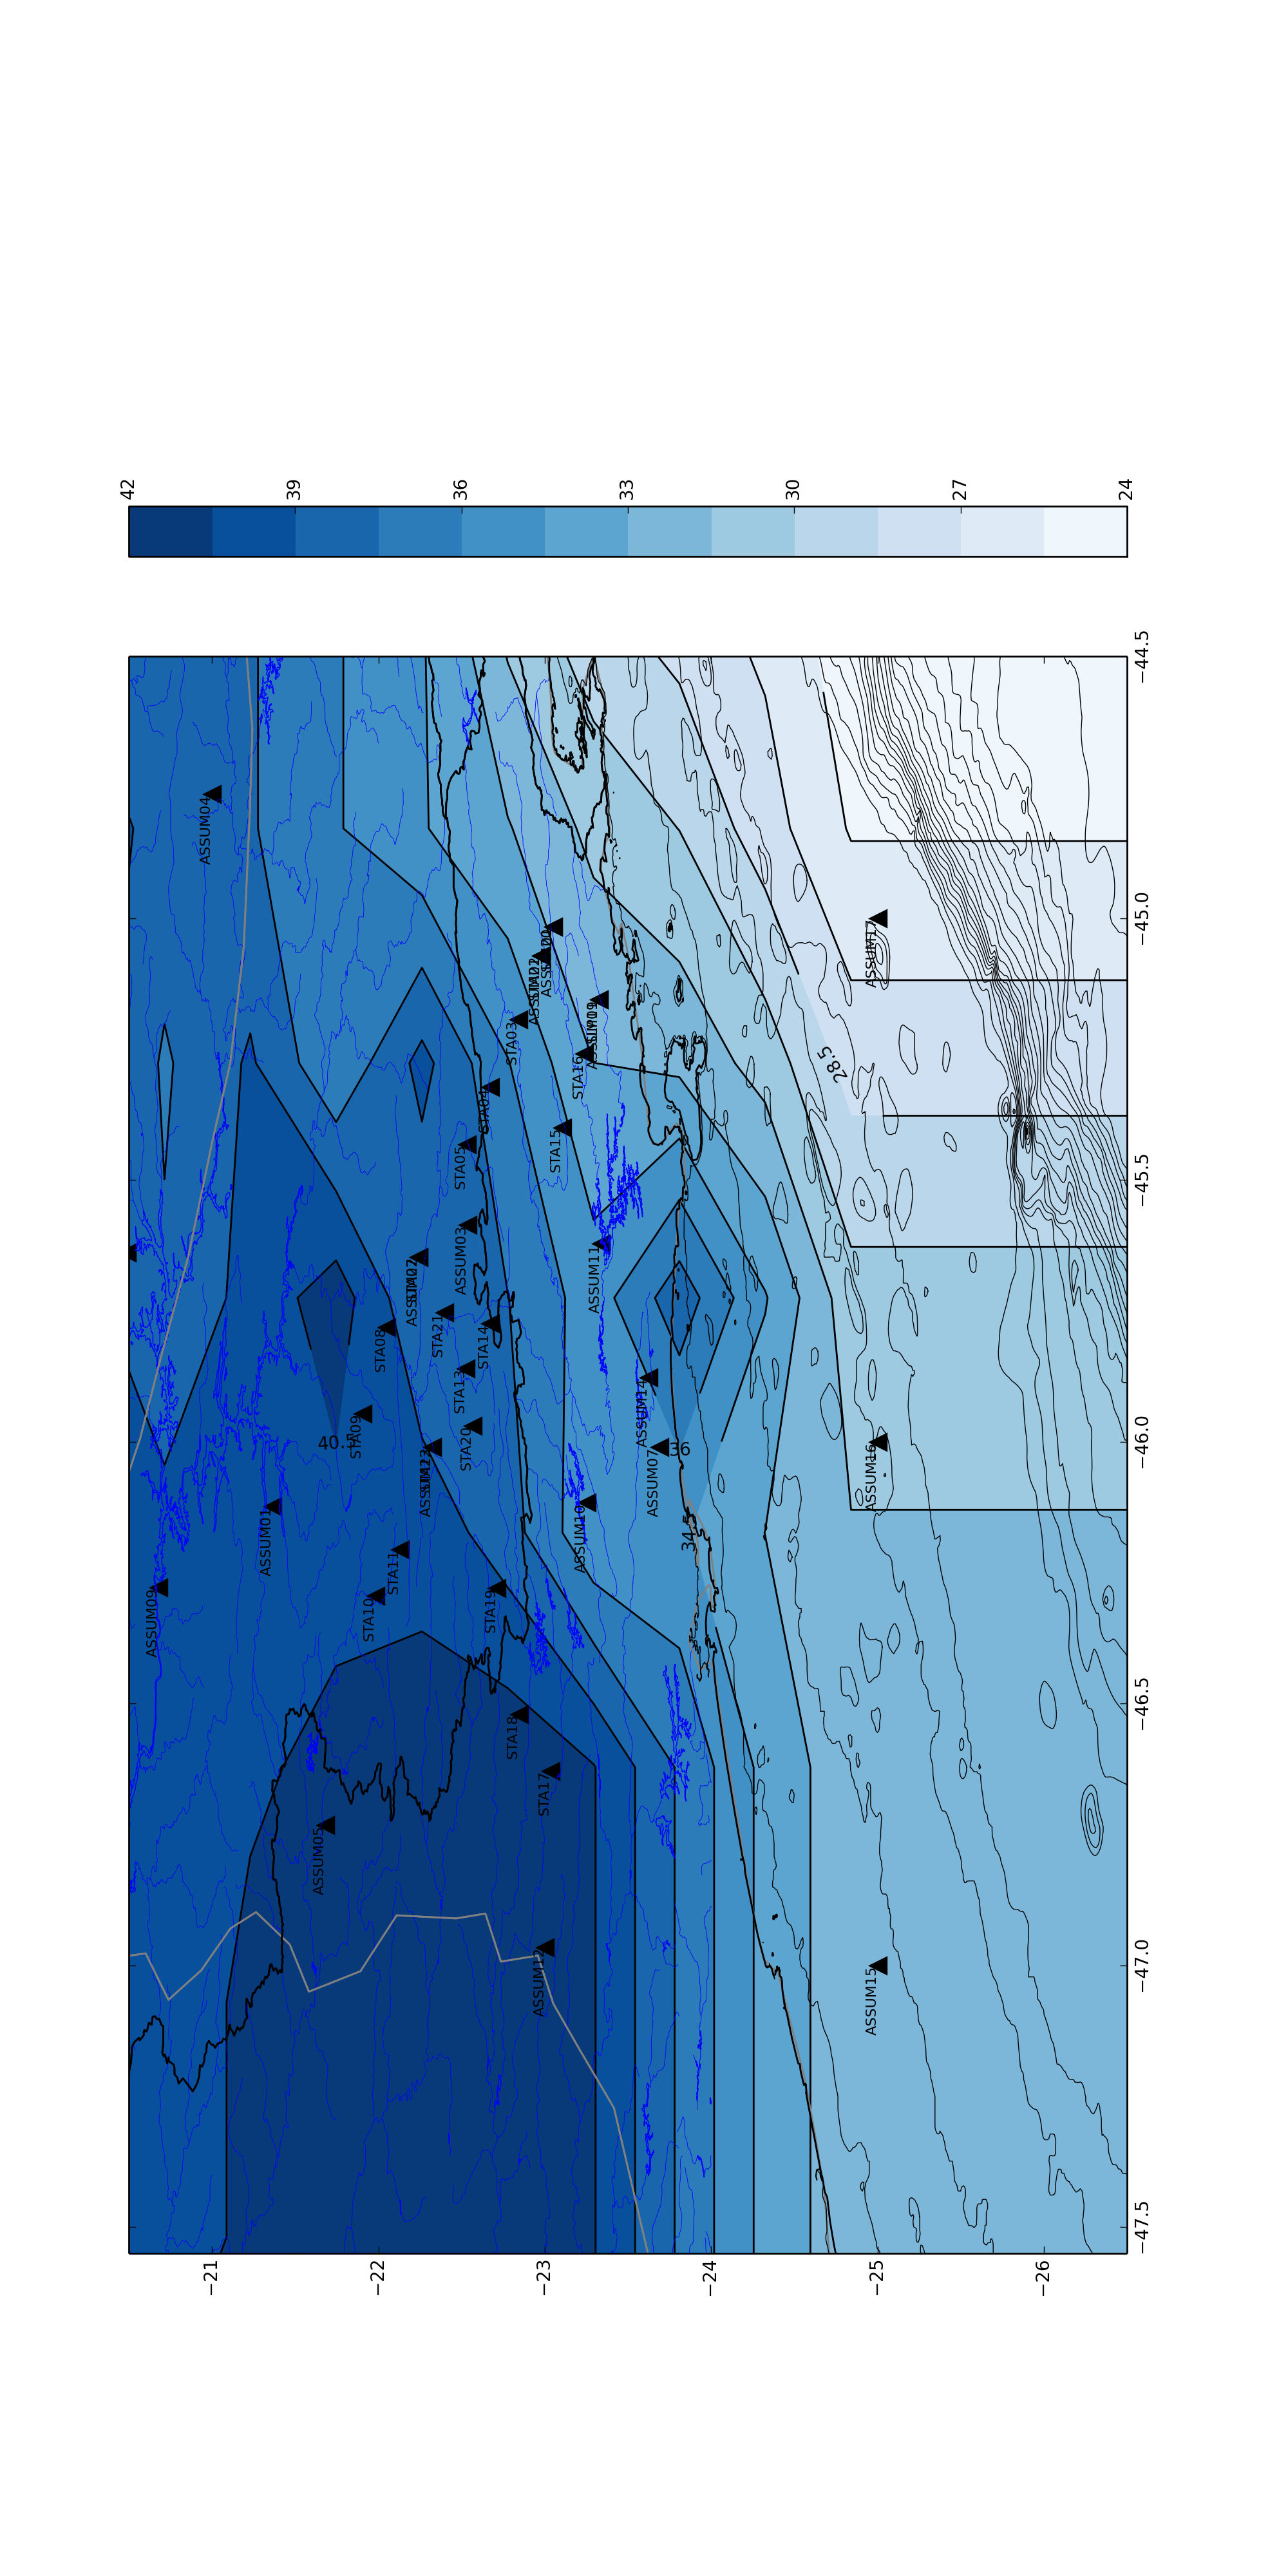
\includegraphics[scale=0.20]{Figs/Interpolacao_Linear.png}
\caption{Mapa da espessura crustal da Faixa Ribeira. Os triângulos representam as estações sismograficas.}
\label{Interpolacao}
\end{figure}

As incertezas na medidas, mostradas na Tabela \ref{tabela1}, estão diretamente ligadas a quantidade e qualidade das Funções do Receptor. A seleção das melhores Funções do Receptor é um fase importante, pois a qualidade da Função do Receptor é prepoderante sobre a quantidade. A imprecisão associada a cada um dos parâmetros obtidos pelo método de \cite{Zhu_Kanamori_2000} é estimada pelo método "\textit{bootstrap}", desenvolvido por \cite{efron_statistical_1991}. Neste trabalho utilizou 200  subconjuntos para se fazer a estimativa das incertezas associadas ao  cálculo da profunidade de Moho e da razão $v_{p}/v_{s}$.

\begin{figure}[!ht]
\centering
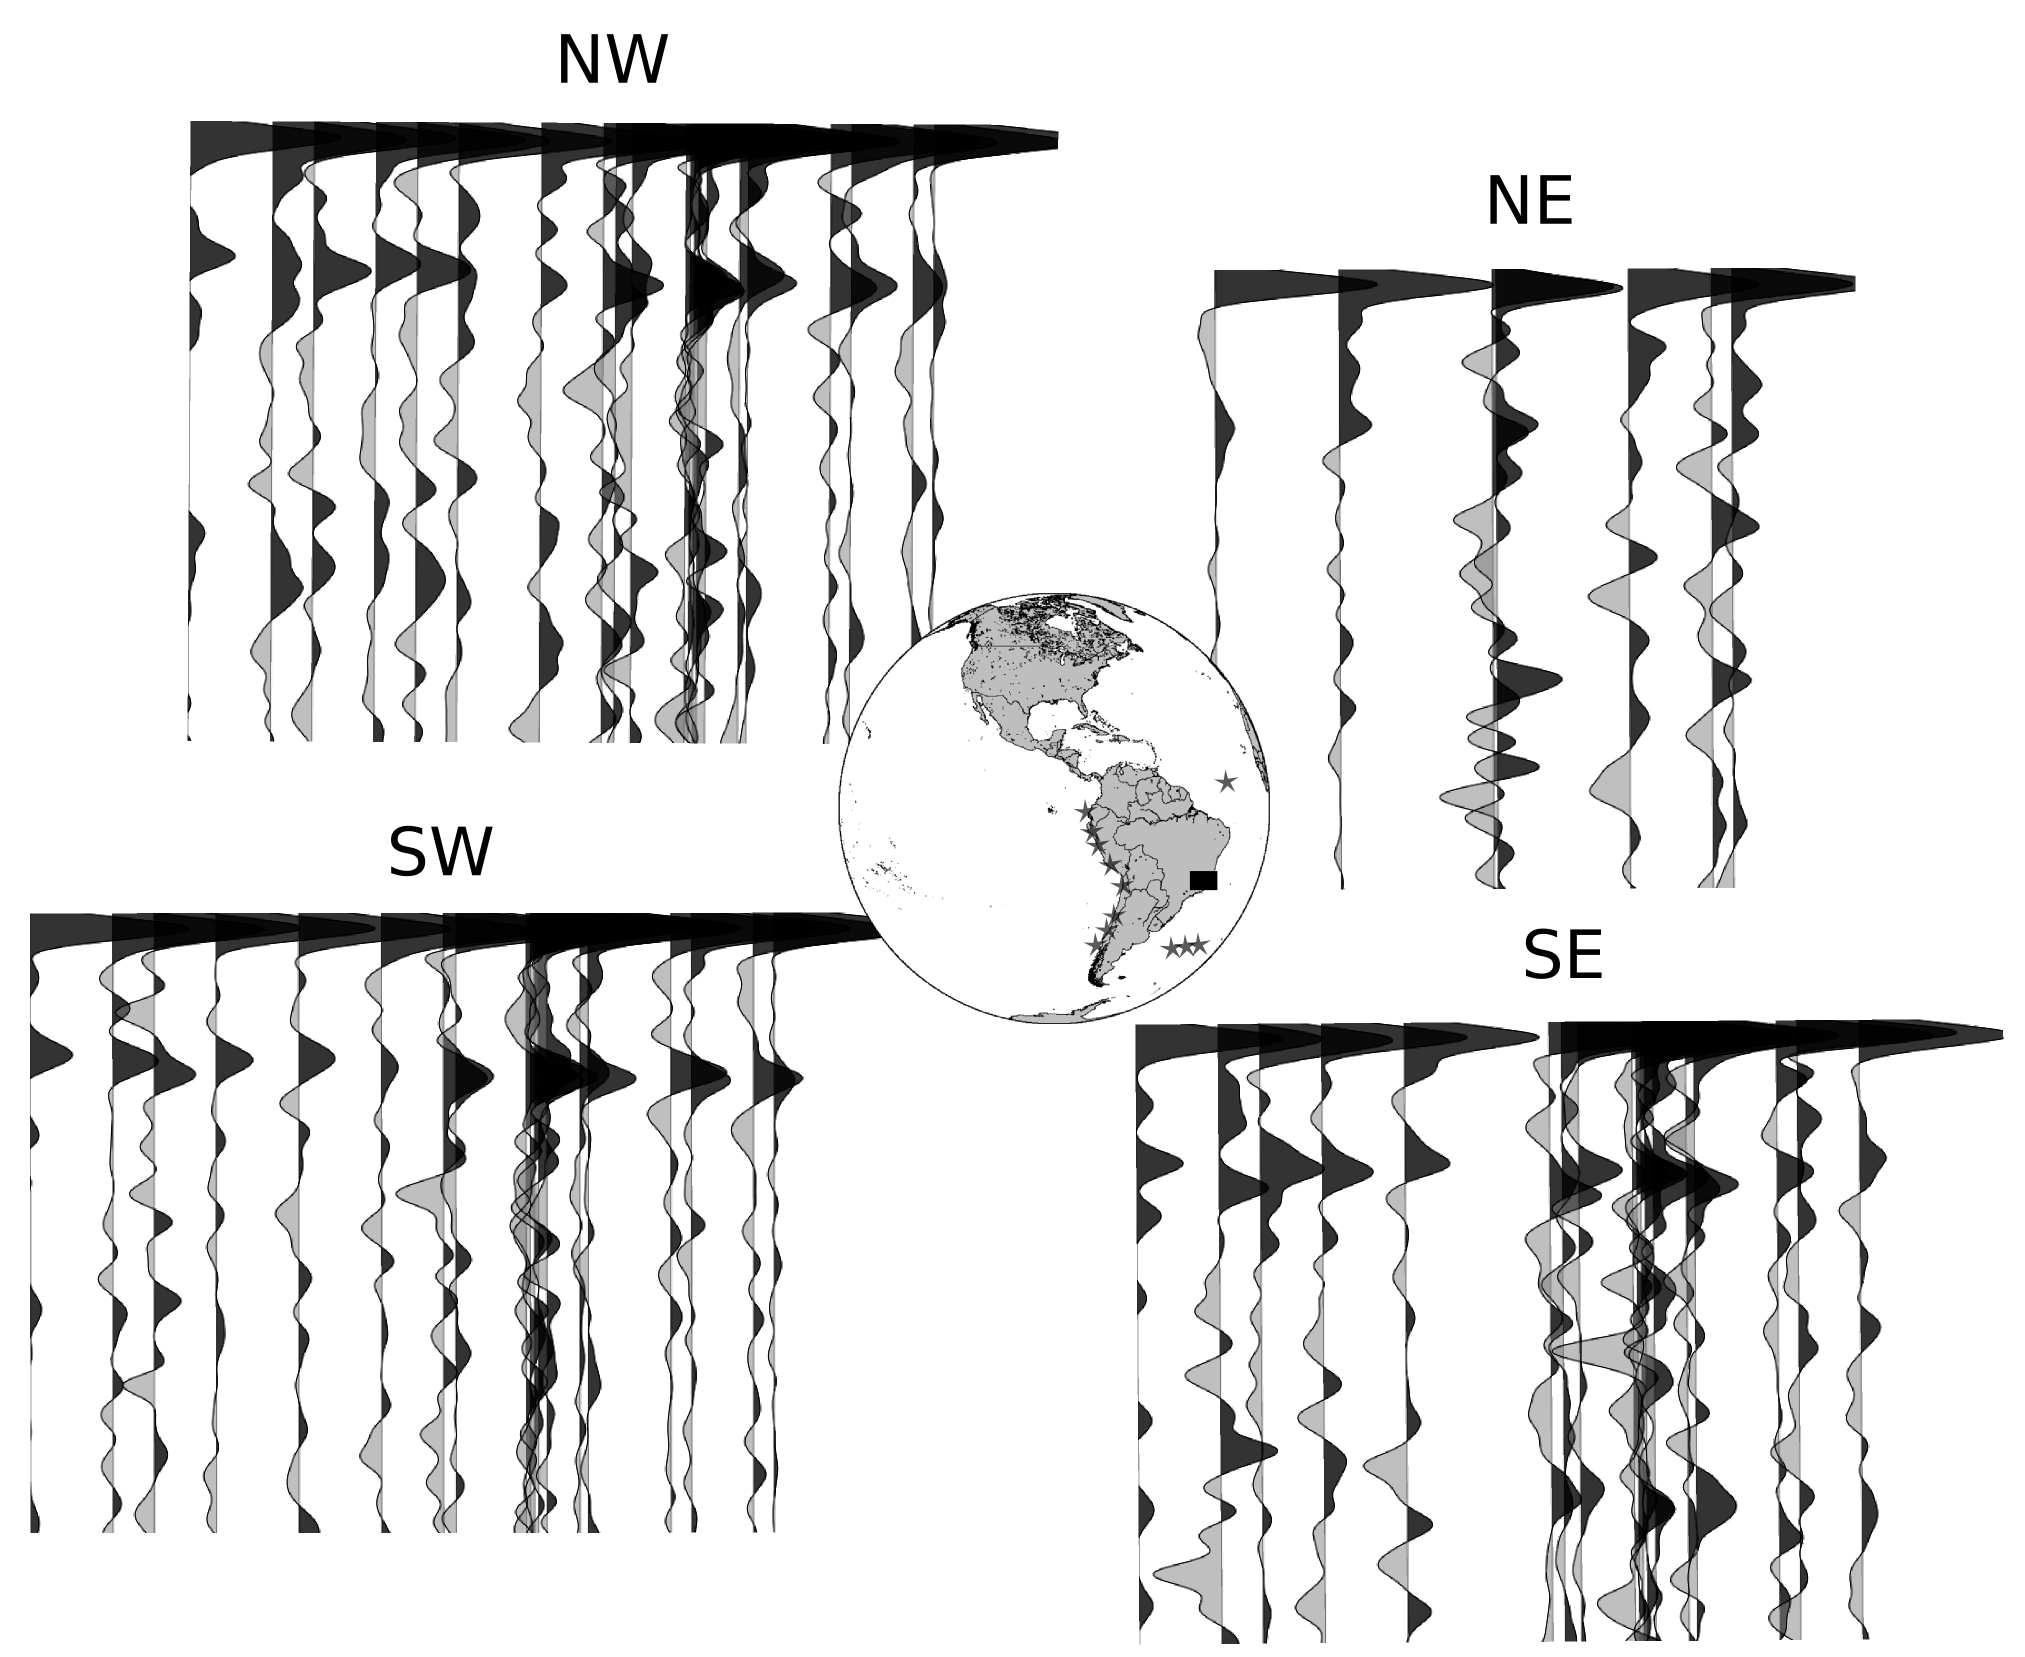
\includegraphics[scale=0.5]{Figs/RF_azimute.png}
\caption{}
\label{RF_perfil_NW}
\end{figure}


%Identfica-se sinais precursores a Moho, por volta de 2 a 4 segundos, que variam ao longo do perfil. Estes sinais podem ser relacionados com uma interface com um alto contraste de propriedade fisica. O pulso negativo antes de 5 segundos indica, segundo as modelagens propostas na Figura \ref{modelagem}, uma camada com baixa velocidade.

\chapter*{Conclusões}	
%\addcontentsline{toc}{chapter}{Referências Bibliográficas}
\bibliographystyle{seg}  
\bibliography{tese_ref}
\chapter*{Anexo 1}	


\begin{center}
\begin{table}[!ht]
\caption{Tabela com as coordenadas(Lat Long) e altitude (m) das Estações.}
\begin{center}
\begin{tabular}{| c | c | c | c |}
\toprule
{\large \textbf{Nome}} &	{\large \textbf{Latitude}} & {\large \textbf{Longitude}} & {\large \textbf{Elevação(m)}}\\
\bottomrule
STA01 & -23.049408 & -45.016808 & 950\\
STA02 & -22.977707 & -45.072017 & 886\\
STA03 & -22.840839 & -45.194141 & 576\\
STA04 & -22.673525 & -45.323162 & 902\\
STA05 & -22.5325 & -45.432383 & 1100\\
STA06 & -22.386261 & -45.549086 & 931\\
STA07 & -22.241667 & -45.647361 & 988\\
STA08 & -22.050056 & -45.781374 & 884\\
STA09 & -21.903929 & -45.946331 & 1045\\
STA10 & -21.98335 & -46.29471 & 1135\\
STA11 & -22.12999 & -46.20536 & 1455\\
STA12 & -22.32379 & -46.01047 & 890\\
STA13 & -22.52571 & -45.86029 & 918\\
STA14 & -22.67147 & -45.77467 & 974\\
STA15 & -23.10378 & -45.39983 & 895\\
STA16 & -23.2387 & -45.25919 & 906\\
STA17 & -23.0337 & -46.62914 & 776\\
STA18 & -22.84539 & -46.52033 & 957\\
STA19 & -22.71192 & -46.27943 & 1413\\
STA20 & -22.56621 & -45.96951 & 908\\
STA21 & -22.39548 & -45.75364 & 957\\
STA22 & -22.21361 & -45.53215 & 1052\\
STA23 & -22.06692 & -45.33267 & 993\\
STA24 & -21.83834 & -44.89324 & 995\\
\hline
\end{tabular}
\label{tabela1}
\end{center}
\end{table}
\end{center}


%\appendix
%\addcontentsline{toc}{chapter}{Apêndice}
%\includepdf[pages={-}]{artigo_sbgf.pdf}$
\end{document}